\twocolumn
\section{Design of an extension of the CWLProv provenance graph}
\label{sec:dev_recommendatons}

\begin{figure*}[ht]
    \centering
    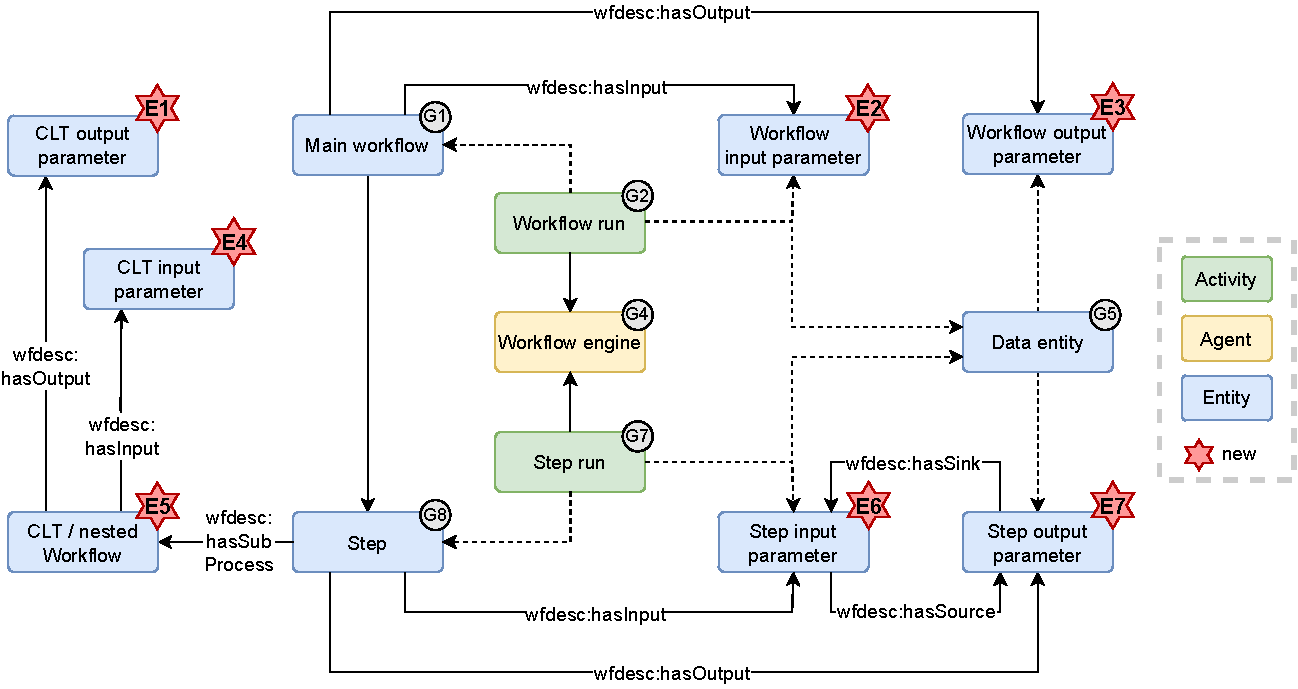
\includegraphics[width=0.99\textwidth]{rdf_extension/CWLProv_graph_extended.pdf}
    \caption{The RDF provenance graph, now extended with \emph{CommandLineTools} and parameter entities. Red stars mark nodes which are part of the design extension. Parameters are linked to their \emph{Workflow}, \emph{CommandLineTool} or step via \emph{wfdesc:hasInput} and \emph{wfdesc:hasOutput}. Node G5 represents both input and output data entities. The data flow between steps is represented via \emph{wfdesc:hasSink} and \emph{wfdesc:hasSource}. Steps are linked to their underlying tools via \emph{wfdesc:hasSubProcess}.}
    \label{fig:cwlprov_graph_new}
\end{figure*}



\begin{figure}[ht]
    \centering
    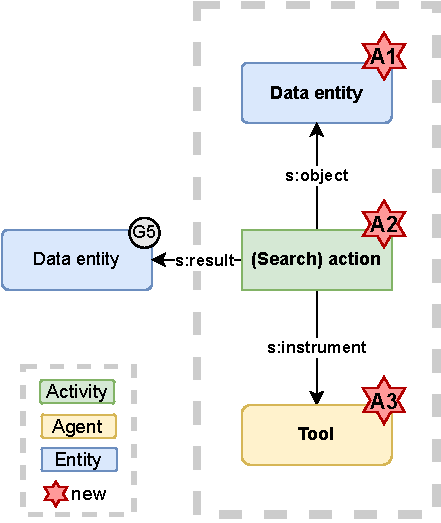
\includegraphics[width=0.4\textwidth]{rdf_extension/CWLProv_graph_extended_actions.pdf}
    \caption{Actions represented in RDF provenance graph. Workflow input datasets (\textbf{G5}) are connected to the Actions (\textbf{A2}) which produced them via \emph{s:result}. In addition, Actions can have properties such as \emph{object} (\textbf{A1}) and \emph{instrument} (\textbf{A3}).  }
    \label{fig:cwlprov_graph_actions}
\end{figure}

In Section \emph{\nameref{sec:cwlprov_evaluation}}, we analyzed CWLProv for the representation of the provenance taxonomy we defined in \emph{\nameref{sec:user_req}}. Based on this analysis, we concluded that not all provenance components were sufficiently represented in a structured format. Specifically, we found that although certain metadata was part of \emph{primary-job.json} and \emph{packed.cwl}, these annotations were not represented in RDF format.

In this section, we propose an extension of the design of the CWLProv provenance graph, which can at least represent the values for already supported metadata fields and can also be extended later with other metadata. %In this way, we (partially) answer \ref{rq:improve}.

Here, we are only concerned with the representation of this information, if it exists. Mechanisms for the collection of the metadata (whether it be manually or automated), are considered out of scope for this paper. 

In Section \emph{\nameref{sec:ext_reqs}}, we first describe the requirements and principles which we used in this design. Subsequently, in Section \emph{\nameref{sec:ext_overview}}, we give a high-level overview of the design. We then give recommendations for specific terms and vocabulary which can be used for the metadata fields \emph{doc}, \emph{label}, \emph{intent}, and \emph{format} which are part of v1.2 of the CWL Standards (Section \emph{\nameref{sec:ext_details}}). We describe how we have partially realized this design in \emph{cwltool} (Section \emph{\nameref{sec:realization}}). Finally, we provide a list of SPARQL queries in Section \emph{\nameref{sup:sparql}}.
\stodor{keep the analysis in?}

\subsection{Requirements and principles}
\label{sec:ext_reqs}
For this design, we reuse principles \ref{pr:bioschemas} and \ref{pr:current_standards}. In addition, the RDF extension should adhere to four requirements.

\begin{enumerate}[label=\textbf{PR\arabic*}]
    \item \label{pr:metadata_fields} Represent the annotations that are supported in CWL workflows according to the CWL standards v1.2, summarized in Table \ref{tab:metadata_fields}.
    \item \label{pr:input} Represent the annotations for \emph{Files} and \emph{Directories} proposed in Section \emph{\nameref{sec:annot_cwl_now}}.
    \item \label{pr:execution} Represent the annotations for a collection of input values proposed in Section \emph{\nameref{sec:annot_cwl_now}}.
    \item \label{pr:actions} Represent the annotations for Actions proposed in Section \emph{\nameref{sec:annot_new_cwl}}.
\end{enumerate}

\subsection{High-level overview}
\label{sec:ext_overview}
In this section, we present a high-level overview of the extended provenance graph and link it to the requirements defined in Section \emph{\nameref{sec:ext_reqs}}.

\subsubsection{Representation of CWL metadata fields}

\begin{table}[bt!]
\caption{Metadata fields in CWL Standards v1.2. \emph{format} is only allowed for parameters of type File or File array.}\label{tab:metadata_fields}
\begin{tabularx}{\linewidth}{L l l l l}
\toprule
Workflow component & label & doc & intent & format \\
\midrule
% Widgets & 42 & Over-supplied\textsuperscript{*} \\
% Gadgets & 13 & Under-supplied \\
Workflow & \textbullet & \textbullet & \textbullet & ~\\ %\hline
WorkflowStep & \textbullet & \textbullet & ~ & ~\\ %\hline
CommandLineTool & \textbullet & \textbullet & \textbullet & ~\\ %\hline
ExpressionTool & ~ & ~ & \textbullet & ~\\ %\hline
WorkflowInputParameter & \textbullet & \textbullet & ~ & \textbullet\\ %\hline
WorkflowOutputParameter & \textbullet & \textbullet & ~ & \textbullet\\ %\hline
WorkflowStepInput & \textbullet & ~ & ~ & ~\\ %\hline
WorkflowStepOutput & ~ & ~ & ~ & ~\\ %\hline
CommandInputParameter & \textbullet & \textbullet & ~ & \textbullet\\ %\hline
CommandOutputParameter & \textbullet & \textbullet & ~ & \textbullet\\ %\hline
\bottomrule
\end{tabularx}
\end{table}

Figure \ref{fig:cwlprov_graph_new} shows how we extended the provenance graph to represent all current metadata fields (\ref{pr:metadata_fields}). \textbf{In the new graph, every workflow component in Table \ref{tab:metadata_fields} is represented as a distinct entity, and interrelated with terms from the \emph{wfdesc} ontology (\ref{pr:bioschemas}).} 
We added entities describing the CWL tools that are run by the steps (\textbf{E5}) and linked them to their input (\textbf{E4}) and output parameters (\textbf{E1}) via \emph{wfdesc:hasInput} and \emph{wfdesc:hasOutput}. We connected the steps (\textbf{G8}) and tools via \emph{wfdesc:hasSubProcess}. In addition, we linked the step parameters (\textbf{E6}, \textbf{E7}) together via \emph{wfdesc:hasSource} and \emph{wfdesc:hasSink} to express the data flow between the steps.

In CWLProv 0.6.0, the execution of nested workflows is described in separate RDF documents. \textbf{Following the same strategy, we recommend to only represent top-level parameters of nested workflows in the primary provenance graph.} More detailed annotations can be represented in the separate RDF documents which describe the nested workflows.

\subsubsection{Representation of input data annotations}
This structure depicted in Figure \ref{fig:cwlprov_graph_new} also supports representation of the input data annotations described in \emph{\nameref{sec:annot_cwl_now}} (\ref{pr:input}), by transferring them to the data entities they describe (\textbf{G5}). 


\subsubsection{Representation of configuration settings annotations} Annotations describing a collection of parameters (\ref{pr:execution}) are specific to the workflow execution. Therefore, we recommend that these annotations are transferred to the entity in the provenance graph describing the workflow execution (\textbf{G2}).

\subsubsection{Representation of input data history}
In the annotation scheme described in Section \emph{\nameref{sec:annot_new_cwl}}, the history of (processed) input data is expressed through \emph{Actions}. Figure \ref{fig:cwlprov_graph_actions} presents their representation in RDF (\ref{pr:actions}). 
Actions (\textbf{A2}) are performed on objects, which are data entities not aggregated in the CWLProv RO (\textbf{A1}). Actions can have additional properties such as Tools (\textbf{A3}) or other annotations as summarized in Table \ref{tab:action_schemaorg}. They are connected to input data entities (\textbf{G5}) via \emph{s:result}. 



\subsection{Details of the design}
\label{sec:ext_details}
Here, we move from the structure of the provenance graph to the annotations that now can be attached to the newly added entities and with which terms they should be represented.

First, we describe which terms to use for the CWL-specific metadata fields \emph{doc}, \emph{label}, \emph{format}, and \emph{intent}.

Although we could use the exact terms with \emph{cwlprov} prefix, we aim for interoperability with other provenance representations, such as the RO-Crate specification. Therefore, we reuse Schema.org terms, and because this is in agreement with our annotation scheme:

\begin{itemize}
    \item \textbf{doc}: http://schema.org/description
    \item \textbf{label}: http://schema.org/name
    \item \textbf{format}: http://schema.org/encodingFormat
    \item \textbf{intent}: http://schema.org/featureList
\end{itemize}

\textbf{In addition, we recommend that custom annotations attached to workflow components and input objects are transferred as they are.} We make an exception for \emph{s:additionalType}, for which the value can be added to the \emph{types} of the entity it describes, instead of being literally transferred as \emph{s:additionalType}.

When entities are described with nested annotations (e.g. \emph{s:citation}), we recommend to make this a separate entity in the graph instead of a nested annotation, in compliance with the PROV data model (\ref{pr:bioschemas}).

\subsection{Partial realization in \emph{cwltool}}
\label{sec:realization}
\todorenske{Update, when this is published there should be full support in cwltool.}
Because of time constraints, we could only partially realize the provenance graph extension in \emph{cwltool}. At the time of writing, annotations directly associated with inputs of type \emph{File} and \emph{Directory}, as exemplified in \emph{\nameref{sec:annot_fair}}, are propagated to the RDF provenance record. However, annotations of the collection of input parameter values (\emph{\nameref{sec:annot_actions}}) or annotations under \emph{cwlprov:prov} (\emph{\nameref{sec:annot_new_cwl}}), are currently not represented in RDF.

\subsection{Conceptual analysis of the design extension}
\label{sec:ext_analysis}

\todorenske{leave in?}
To test the extended design, we analyzed the RDF provenance graph which would have been associated with the epitope prediction workflow we used as an example in this thesis. The elements of the design which were not yet realized in \emph{cwltool}, we emulated via manual annotations of the document. 

\subsubsection{SPARQL queries.}

\todorenske{replace with all sparql queries}
Here, we present two example SPARQL queries we issued on the emulated extended provenance graph. The first (\textbf{Q1}) extracts the DOIs of all publications which were the citations of the used inputs.

The second (\textbf{Q2}) lists the formats for every file for which this is specified.